\section{Introduction}
\label{sec:intro}

Galois field (GF) arithmetic is part of modern abstract algebra focused on 
computations on modulo-based fields
and finds application in areas such as 
cryptography, error control coding, VLSI testing, etc. In most
hardware applications, fields of the type $\Fkk$ are widely
chosen. Such { binary} GFs are $k$-dimensional extensions
of the base field ${\mathbb{F}}_2$; this allows for the design of
efficient (AND-XOR) arithmetic architectures and algorithms for
hardware design. Due to their deployment in communications and
security-related applications, there is a critical need to {
  formally verify} the correctness of hardware implementations of GF
arithmetic. In most applications, however, the datapath size
(bit-vector operand size) $k$ is too large to use naive enumeration test. Most conventional formal
verification methods are unable to cope with the large size and
complexity of GF circuits. 

GF arithmetic circuits in $\Fkk$ take $k$-bit vectors as inputs and
produce $k$-bit outputs. For example, a GF modulo multiplier computes
$R = A \times B \pmod{ P(x)}$, where: i) $A = a_{s(0)} + a_{s(1)}\alpha +
\dots + a_{s(k-1)} \alpha^{k-1} = \sum _{i=0}^{k-1} a_{s(i)}\alpha^i$,
$B = \sum_{i=0}^{k-1}b_{s(i)} \alpha^{i}$ denote the $k$-bit inputs,
$R = \sum _{i=0} ^{k-1} r_{s(i)} \alpha^i$ is the output, and $a_{s(i)},
b_{s(i)}, r_{s(i)} \in \Ftwo$; ii) $P(x)$ is the given primitive
polynomial used to construct $\Fkk$; and iii) $P(\alpha) = 0$,
i.e, $\alpha$ is the primitive element of the field. In the above, the
elements are represented in { standard basis notation} (denoted by
subscript ``s'' on the bits). As the datapath size $k$ increases,
combinational GF designs become prohibitively large;
%\cite{wu:2002} \cite{acar:1998}; 
sequential GF circuits are therefore desirable. 

Sequential GF circuits operate as follows: $k$-bit input operands are
loaded into $k$-bit state registers (flip-flops), and the circuit is
executed for $k$ clock-cycles; after which the $k$-bit result is
available in the output registers. Data representation and circuit
design for sequential GF circuits is mostly based on { normal basis}
\cite{gao:phd_normal_basis}. Data is represented as $A = a_{n(0)}
\beta + a_{n(1)} \beta^2 + a_{n(2)} \beta^{2^2} + \dots + a_{n(k-1)}
\beta^{2^{k-1}}$, where $\beta \in \Fkk$ is the { normal
  element}, and $\{\beta, \beta^2, \dots, \beta^{2^i}, \dots,
\beta^{2^{k-1}}\}$ forms the normal basis. Standard and normal basis
representations can be derived from each other, i.e, $\beta$ can be
derived from $\alpha$ and vice-versa. It has been shown that
architectures for multiplication and  squaring can be efficiently
designed using normal bases  \cite{agnew1991implementation} 
\cite{RHmulti} \cite{gao:phd_normal_basis} as sequential circuits. 
\footnote{In fact, some (not all) finite fields have an
  { optimal normal basis}, where the combinational logic part of
  the sequential circuit contains a minimum number of 2-input AND/XOR
  gates.}.

\begin{Example}
\label{ex:nb_sq}
For $a, b \in \Fkk, (a+b)^2 = a^2 + b^2$. Applying this rule for
element squaring: 
\begin{align}
B = & (b_0\beta + b_1\beta^2 + b_2\beta^4 + \dots + b_{k-1}\beta^{2^{k-1}}) \nonumber\\
B^2 = &b_0^2\beta^2 + b_1^2\beta^4 + b_2^2\beta^8 + \dots + b_{k-1}^2\beta^{2^k} \nonumber\\
= &b_{k-1}\beta + b_0\beta^2 + b_1\beta^4 + \dots + b_{k-2}\beta^{2^{k-1}} \nonumber
\end{align}
as $\beta^{2^k} = \beta$ due to Fermat's little theorem, and $b_i^2 = b_i$. 
\end{Example}

The above example shows that squaring of elements represented in
normal bases can be implemented simply by a cyclic right-shift
operation. However, multiplication of two elements in normal basis is
still a complicated operation --- and its design and verification is still
challenging. Recent literature has addressed formal equivalence proofs
of { combinational} GF arithmetic circuits \cite{ibm:blueveri}
\cite{lv:tcad2013} \cite{pruss:dac14}. Our research aims to address verification
of sequential GF circuits, which has not been addressed before. 


{\it Problem Statement:} We are given: 
i) the Galois field $\Fkk = \Ftwo[X] \pmod{ P(X)}, P(\alpha) = 0$,
along with the { normal basis representation}, i.e. $\beta$ is also
known; 
ii) a word-level specification polynomial $R = \F(A, B) \pmod{ P(X)}$;
where $A = \sum _{i=0}^{k-1} a_i \beta^{2^{i}}$, $B = \sum
_{i=0}^{k-1} b_i \beta^{2^{i}}$, $R = \sum _{i=0}^{k-1} r_i
\beta^{2^{i}}$, $ a_i, b_i, r_i \in \Ftwo$, and iii) a sequential
circuit ($S$) implementation of the 
polynomial computation. Our objective is to prove or disprove that $S$
is a $k$-cycle implementation of $R$. 

{\it Approach \& Contributions:} The sequential GF arithmetic circuit
can be viewed as a {restricted} Mealy finite state machine (FSM),
as shown in Fig. \ref{fig:sequential}. The FSM contains no
primary inputs or outputs. The operands are loaded into state
registers $A, B$ (as initial states), and after $k$-clock cycles of
operation, the result $R = \F(A, B)$ is stored in the $R$ register. 

\begin{figure}[htb]
\begin{center}
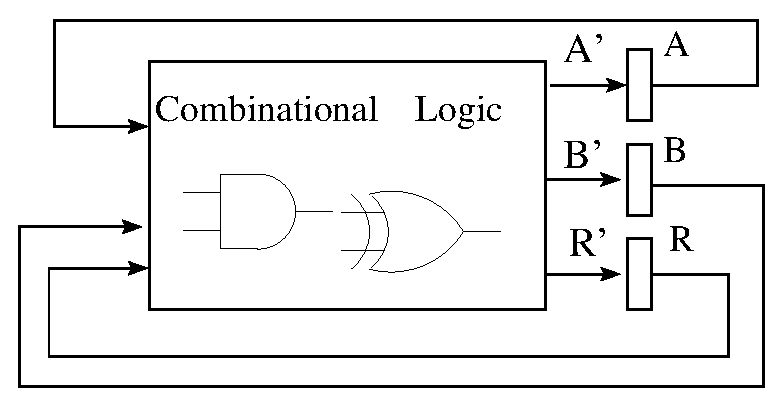
\includegraphics[width=2.8in]{./gf_seq_model.eps}
\end{center}
\caption{\small A typical normal basis GF sequential circuit model. $A =
  (a_0,\dots,a_{k-1})$ and similarly $B, R$ are $k$-bit registers;
  $A', B', R'$ denote next-state inputs.}
\label{fig:sequential}
\end{figure}

% \vspace{-0.2in}
A straightforward approach to verify such a sequential circuit may
consist of unrolling the circuit for $k$ time-frames, and performing a
(combinational) equivalence check between the unrolled machine and the
specification polynomial. Such a technique is grossly inefficient for
large circuits. Therefore, we propose a method that implicitly
(symbolically) represents the unrolled computation, { canonically,
  as a word-level multi-variate polynomial.} We show that the
$k$-cycle polynomial representation can be derived { iteratively}
by performing a sequence of \Grobner basis ($GB$) computations of the
ideal generated by the polynomials corresponding to the circuit. The
approach  requires the use of a specific elimination term order for
the $GB$ computation, based on the circuit's topology. Once the
canonical polynomial is derived, it can be checked against the
specification polynomial for verification.  

Computing \Grobner bases with elimination orders is infeasible for
large circuits. To overcome this complexity, we draw inspiration from
\cite{pruss:dac14}, and exploit the binomial expansion in GFs to
engineer a new, efficient implementation to derive the word-level
polynomial. We demonstrate the feasibility of our approach by
verifying (and also detecting bugs in) up to 100-bit sequential GF
multipliers (containing 300 flip-flops), whereas conventional
techniques fail beyond 23-bit circuits. Finally, our approach can be
construed as a word-level, implicit traversal of the underlying FSM of
the sequential GF circuit, wherein the set of states is encoded as the
variety of an elimination ideal related to the FSM transition
function.  

